\documentclass[a4paper]{fhnwreport} %Legt grundlegende Formatierungen wie Schriftarten, Ort Seitenzahlen etc. fest.

\usepackage[overload]{empheq}
\usepackage{pdfpages}
\usepackage{listings}
\usepackage{color}
\usepackage{amssymb}

\newcommand*{\widebox}[2][0.5em]{\fbox{\hspace{#1}$\displaystyle #2$\hspace{#1}}}
\title{Formelsammlung dglE}
\author{The Procrastinators}
\graphicspath{{./graphics/}}%Change according to graphics folder!

\definecolor{matlab-comments-color}{RGB}{28,172,0} % color values Red, Green, Blue
\definecolor{matlab-string-color}{RGB}{170,55,241}

\begin{document}
    \lstset{language=Matlab,%
       %basicstyle=\color{red},
        breaklines=true,%
        morekeywords={matlab2tikz},
        keywordstyle=\color{blue},%
        morekeywords=[2]{1}, keywordstyle=[2]{\color{black}},
        identifierstyle=\color{black},%
        stringstyle=\color{matlab-string-color},
        commentstyle=\color{matlab-comments-color},%
        showstringspaces=false,%without this there will be a symbol in the places where there is a space
        numbers=left,%
        numberstyle={\tiny \color{black}},% size of the numbers
        numbersep=9pt, % this defines how far the numbers are from the text
        emph=[1]{for,end,break},emphstyle=[1]\color{red}, %some words to emphasise
        %emph=[2]{word1,word2}, emphstyle=[2]{style},   
    }

    \maketitle
    \section{Sonstiges}
\subsection{Häufig verwendete Integrale}
\begin{flalign*}
    & \int \frac{f'(x)}{f(x)} = \ln\lvert f(x)\lvert + c \\
    & \int ln(x)dx = \left|\begin{array}{llrr}
                                u  &= ln(x) & u' &= \frac{1}{x} \\
                                v' &= 1     & v  &= x           \\
                            \end{array}\right| = x\,ln(x) - \int\,dx = x\left(ln(x)-1\right) + c \\
\end{flalign*}

    \subsection{RLC Definitionen}

\begin{align*}
    \textrm{R:}\hspace{5mm} & u(t) = R \cdot i(t)             & i(t) &= \frac{u(t)}{R} \\
    \textrm{C:}\hspace{5mm} & u(t) = \frac{1}{C}\int i(t)dt+c & i(t) &= \frac{du}{dt}C \\
    \textrm{L:}\hspace{5mm} & u(t) = \frac{di}{dt}L           & i(t) &= \frac{1}{L}\int u(t)dt+c \\
\end{align*}


    \section{Separabel}
\begin{align*}
y' &= \frac{d y}{d x} \\
&= f(x)\cdot g(y)\\
&\Downarrow\\
\frac{d y}{g(y)} &= f(x)d x\\
\int{\frac{d y}{g(y)}} &= \int{f(x)d x}\\
F_{1}(y) &= F_{2}(x)+C \qquad C\Rightarrow y(x_{0}) = y_{0}
\end{align*}
    \section{Substitution}

\begin{center}
\begin{align*}
y' &= f(ax+by+c) \\
&\Downarrow \\
u &= u(x) = ax +by +c\\
\frac{du}{dx} &= a + b\frac{dy}{dx}\\
\frac{du}{dx} &= a +b\cdot u\\
\frac{du}{a+b\cdot u} &= dx\\
&\Downarrow \text{Variablentrennung}\\
y &= \frac{u-a-c}{b}
\end{align*}
\end{center}

\begin{center}
\begin{align*}
y' &= f\left(\frac{y}{x}\right)\Rightarrow u =\frac{y}{x}\\
y &= u\cdot x\\
y' &= u'\cdot x + u \Rightarrow f(u) = u'\cdot x +u\\
\frac{du}{dx} &= \frac{f(u)-u}{x}\\
&\Downarrow \text{Variablentrennung}\\
u &= u(x) \Rightarrow u = \frac{y}{x}\\
y &= u(x)\cdot x
\end{align*}
\end{center}

    \newpage
    \section{Eulerverfahren}

\begin{equation*}
    \textrm{Sei}\hspace{3mm} y' = \frac{dy}{dx} = f(x, y)
\end{equation*}

\begin{align*}
    \textrm{Mit Taylor: } &  y(x)\approx y_0 + y'(x_0)(x-x_0) \approx y_0 + f(x_0,y_0)(x-x_0) & \textrm{(gilt nur wenn $(x_0,y_0)$ klein ist)} \\
                          & x-x_0 = h \hspace{5mm}\rightarrow\hspace{5mm} x = x_0 + h & \\
                          & y(x_0 + h) \approx y_0 + f(x_0,y_0) \cdot h & \\
\end{align*}

Meistens gegeben sind:
\begin{align*}
    P_0 &= (x_0,y_0) \hspace{5mm}\textrm{aka}\hspace{5mm} y(x_0)=y_0             & \textrm{Anfangswert} \\
    x   &\in [x_0, x_m] \hspace{5mm}\textrm{aka}\hspace{5mm} \Delta x=x_m-x_0    & \textrm{Schrittgr\"osse}\\
    n   &                                                  & \textrm{Anzahl Iterationen}\\
    h   &= \frac{\Delta x}{n}                              & \textrm{Schritth\"ohe}\\
\end{align*}

Das Verfahren:
\begin{align*}
    \begin{rcases}
        x_1 &= x_0 + h \\
        y_1 &= y_0 + m_0 h = y_0 + h\cdot f(x_0,y_0) \\
    \end{rcases} P_1(x_1,y_1) \\
    \begin{rcases}
        x_2 &= x_1 + h \\
        y_2 &= y_1 + m_1 h = y_1 + h\cdot f(x_1,y_1) \\
    \end{rcases} P_2(x_2,y_2) \\
    \begin{rcases}
        \ldots \\
    \end{rcases} P_3(x_3,y_3) \\
\end{align*}
\begin{equation*}[box=\widebox]
y_{n}=y_{n-1}+h\cdot f\left(x_{n-1},y_{n-1}\right)
\end{equation*}


    \newpage
    \section{Allgemeine L\"osung Lineare DGL 1. Ordnung}

Eine Differentialgleichung ist linear, wenn sie in der folgenden Form dargestellt werden kann:

\begin{align*}
    y'+p(x)\cdot y = r(x)\begin{cases}
r(x) = 0 \qquad\text{homogene lineare DGL 1.Ordnung}\\
r(x) \neq 0 \qquad \text{inhomogene lineare DGL 1.Ordnung}
\end{cases}
\end{align*}

\subsection{homogene lineare DGL 1.Ordnung}

\begin{align*}
    y' + p(x)\cdot y            &= 0                  \\
    \frac{dy}{dx} + p(x)\cdot y &= 0                  \\
    \int\frac{dy}{y}            &= -\int p(x)dx       ,\hspace{8mm}y \neq 0 \\
    ln\lvert y\lvert            &= -\int p(x)dx + c   \\
\end{align*}

\begin{equation*}[box=\widebox]
    y(x) = Ke^{-\int p(x)dx}       \hspace{8mm} K\in{\rm I\!R}
\end{equation*}

\subsection{inhomogene lineare DGL 1.Ordnung}

$y' + p(x) \cdot y = r(x) \rightarrow$ Verfahren ``Variation der Konstanten'':
\begin{align*}
    y_p(x)             &= K(x)e^{-\int p(x)dx} \\
    y_p'(x)            &= K'(x)e^{-\int p(x)dx} - K(x)p(x)e^{-\int{p(x)dx}} \\
                       &\rightarrow r(x) = y' + p(x) \cdot y \\
    r(x)               &= K'(x)e^{-\int p(x)dx} - K(x)p(x) - K(x)p(x)e^{-\int p(x)dx} + p(x)K(x)e^{-\int p(x)dx} \\
    r(x)               &= K'(x)e^{-\int p(x)dx} \\
    K'(x)              &= r(x)e^{\int p(x)dx} \\
    K(x)               &= \int r(x)e^{\int p(x)dx} \\
    \Rightarrow y_p(x) &= K(x)e^{-\int p(x)dx} = \left(\int r(x)e^{\int p(x)dx}\right) \cdot e^{-\int p(x)dx} \\
\end{align*}

\begin{equation*}[box=\widebox]
    y(x) = C \cdot e^{-\int p(x)dx} + e^{-\int p(x)dx} \int r(x)e^{\int p(x)dx}dx
\end{equation*}


    \section{Bernoullische Differentialgleichung}

\begin{align*}
y'+p(x)\cdot y = r(x)y^{s}\qquad s\neq\{0,1\}\\
y^{-s}y' + p(x)y^{1-s} = r(x)\Rightarrow z=y^{1-s}\\
z'=(1-s)y^{-s}y'\Rightarrow y^{-s}y'=\frac{z'}{1-s}\\
\Longrightarrow \boxed{z'+(1-s)p(x)z= (1-s)r(x)}
\end{align*}
    \section{DGL 2. Ordnung}
\subsection{homogen}

\begin{align*}
&y'' + ay' +by = 0\\
&\Rightarrow \lambda^2 +a\lambda+b=0 \\
&D =  a^2-4b
\end{align*}


\begin{align*}
\text{Fall $D>$ 0:\qquad}\lambda_{1,2} &= \frac{-a\pm\sqrt{a^2-4b}}{2}\\
y(x) &= C_{1}e^{\lambda_{1}x}+C_{2}e^{\lambda_{2}x}
\end{align*}

\begin{align*}
\text{Fall $D=$ 0:\qquad}\lambda_{0} &= -\frac{a}{2}\\
y(x) &= C_{1}e^{\lambda_{0}x}+xC_{2}e^{\lambda_{0}x}
\end{align*}

\begin{align*}
\text{Fall $D<$ 0:\qquad}\lambda_{1,2} &= -\frac{a}{2}\pm \frac{j\sqrt{4b-a^2}}{2}
=\alpha\pm j\beta
\begin{cases}
\alpha = -\frac{a}{2}\\
\beta = \frac{\sqrt{4b-a^2}}{2}
\end{cases}\\
y(x) &= e^{\alpha x}\left[k_{1}\cos(\beta x)+k_{2}\sin(\beta x)\right]
\end{align*}



    \section{Funktionen mehrerer Variablen}

\subsection{Matlab}

This shit will plot a function with mehrere Variables.
\lstinputlisting{./matlab/meshgrid.m}

Niveaulinien plotten:
\lstinputlisting{./matlab/niveaulinien.m}


\subsection{Ebene}

Eine Ebene kann mit der folgenden allgemeinen Gleichung beschrieben werden.
\begin{equation*}
    ax + by + cz + d = 0
\end{equation*}

Die r\"aumliche Lage einer Ebene mit der allgemeinen  Funktionsgleichung l\"asst
sich aus ihren Schnittpunkten $S_x$, $S_y$, $S_z$ mit den drei Koordinatenachsen
bestimmen.

\begin{align*}
    S_x &= \left(-\frac{d}{a}, 0, 0\right) &
    S_y &= \left(0, -\frac{d}{b}, 0\right) &
    S_z &= \left(0, 0, -\frac{d}{c}\right) \\
\end{align*}


\subsection{Grenzwert}

Beispiel:
\begin{align*}
    f(x,y) &= \frac{xy}{x^2+ y^2} & \\
    \lim_{(x_0,y_0) \to (0,0)} f(x,y) &= \lim_{x \to 0} f(x,mx) \\
    &= \frac{m}{1+m^2} \\
\end{align*}


\subsection{Polarkoordinaten}

\begin{align*}
    x &= r \cos \theta \\
    y &= r \sin \theta \\
    f(x,y) &= \frac{xy^2}{x^2 + y^4} \\
    \lim_{(x,y) \to (0,0)} \frac{xy^2}{x^2 + y^4} &= \lim_{r \to 0} \frac{r\cos\theta\sin^2\theta}{\cos^2(\theta) + r^2\sin^4(\theta)} \\
\end{align*}



    \section{Niveaulinie/Grenzwertbestimmung}

\begin{align*}
z = f(x,y) \Rightarrow z = c\\
\text{nach y auflösen und mit Matlab plotten}\\
D_{f} = \left\{x,y\in\mathbb{R}, f(x,y)\right\}
\end{align*}

\begin{align*}
f(x,y) = 0 \quad&\text{für}\quad (x,y) = (0,0)\\
\text{Überprüfen ob Grenzwert existiert: } &\lim\limits_{r \to 0} f(r\cos(\Theta),r\sin(\Theta) 
\end{align*}

    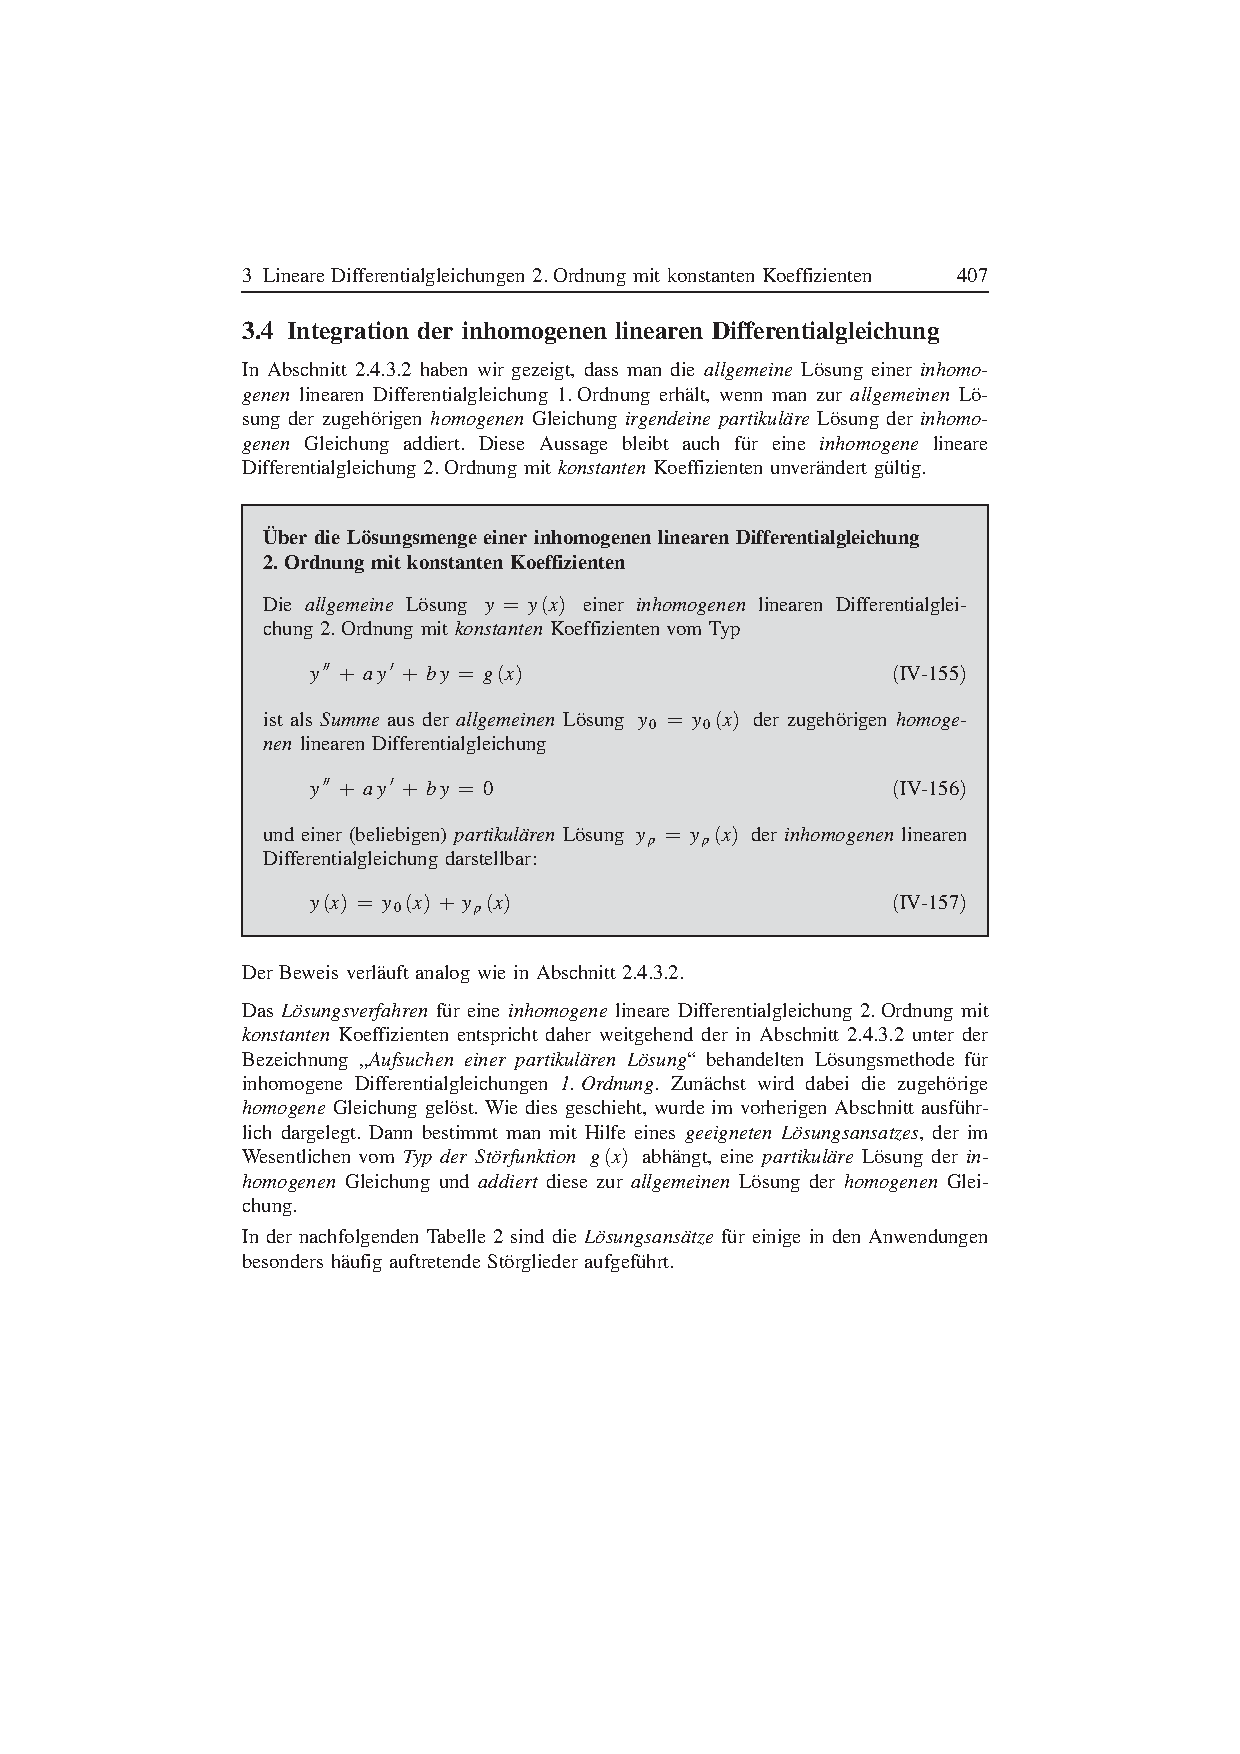
\includepdf[pages=-]{./sections/dglE_inhomogen.pdf}
\end{document}
